\documentclass[tikz,border=5mm]{standalone}
\usetikzlibrary{patterns}
\begin{document}
	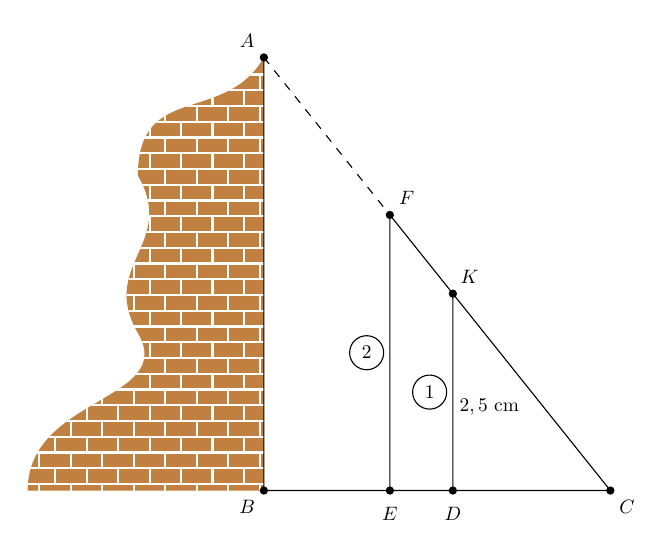
\begin{tikzpicture}[nodes={scale=.7}]
		\path
		(0,0) coordinate (D)
		(0,2.5) coordinate (K)
		(2,0) coordinate (C)
		(C)--(K) coordinate[pos=1.4] (F) coordinate[pos=2.2] (A)
		(C)--(D) coordinate[pos=1.4] (E) coordinate[pos=2.2] (B)
		;
		% miền tường gạch
		\def\brickwall{
			(B)--++(-3,0)
			.. controls +(90:1.2) and +(-60:1) .. (-4,2)
			.. controls +(120:1) and +(-60:1) .. (-4,4)
			.. controls +(90:1.2) and +(-120:1) .. (A)
		}
		\fill[brown] \brickwall;
		\pattern[pattern color=white,pattern=bricks] \brickwall;
		\draw[dashed] (A)--(F);
		\draw (A)--(B)--(C)--
		(F)--(E) node[pos=0.5,left=3pt,circle,draw]{$2$}
		(D)--(K) node[pos=0.5,left=3pt,circle,draw]{$1$}
		node[pos=0.5,below right]{$2,5$ cm};
		\foreach \p/\goc in {A/135,B/-135,C/-45,D/-90,E/-90,F/45,K/45}
		\fill (\p) circle(1.5pt) +(\goc:.3) node{$\p$};
	\end{tikzpicture}
\end{document}